%; whizzy paragraph -pdf xpdf -latex ./whizzypdfptex.sh
%; whizzy-paragraph "^\\\\begin{frame}"
% latex beamer presentation.
% platex, latex-beamer $B$G%3%s%Q%$%k$9$k$3$H$rA[Dj!#(B 

%     Tokyo Debian Meeting resources
%     Copyright (C) 2009 Junichi Uekawa
%     Copyright (C) 2009 Nobuhiro Iwamatsu

%     This program is free software; you can redistribute it and/or modify
%     it under the terms of the GNU General Public License as published by
%     the Free Software Foundation; either version 2 of the License, or
%     (at your option) any later version.

%     This program is distributed in the hope that it will be useful,
%     but WITHOUT ANY WARRANTY; without even the implied warranty of
%     MERCHANTABILITY or FITNESS FOR A PARTICULAR PURPOSE.  See the
%     GNU General Public License for more details.

%     You should have received a copy of the GNU General Public License
%     along with this program; if not, write to the Free Software
%     Foundation, Inc., 51 Franklin St, Fifth Floor, Boston, MA  02110-1301 USA

\documentclass[cjk,dvipdfm,12pt]{beamer}
\usetheme{Tokyo}
\usepackage{monthlypresentation}

%  preview (shell-command (concat "evince " (replace-regexp-in-string "tex$" "pdf"(buffer-file-name)) "&"))
%  presentation (shell-command (concat "xpdf -fullscreen " (replace-regexp-in-string "tex$" "pdf"(buffer-file-name)) "&"))
%  presentation (shell-command (concat "evince " (replace-regexp-in-string "tex$" "pdf"(buffer-file-name)) "&"))
%  presentation (shell-command (concat "evince " (replace-regexp-in-string "tex$" "pdf"(buffer-file-name)) "&"))

%http://www.naney.org/diki/dk/hyperref.html
%$BF|K\8l(BEUC$B7O4D6-$N;~(B
\AtBeginDvi{\special{pdf:tounicode EUC-UCS2}}
%$B%7%U%H(BJIS$B7O4D6-$N;~(B
%\AtBeginDvi{\special{pdf:tounicode 90ms-RKSJ-UCS2}}

\title{Why GPG Key sign?}
\subtitle{$BEl5~%(%j%"(B Debian $BJY6/2q(B in OSC 2009 Tokyo/Fall}
\author{$B4d>>(B $B?.MN(B iwamatsu@debian.or.jp\\IRC nick: iwamatsu}
\date{2009$BG/(B10$B7n(B31$BF|(B}
\logo{
\includegraphics[width=8cm]{image200607/openlogo-light.eps}}

%begin of commandline0
\newenvironment{commandline0}%
{\VerbatimEnvironment
  \begin{Sbox}\begin{minipage}{0.95\hsize}\begin{fontsize}{9}{9} \begin{BVerbatim}}%
{\end{BVerbatim}\end{fontsize}\end{minipage}\end{Sbox}
  \setlength{\fboxsep}{10pt}

\vspace{10pt}% skip before
\fcolorbox{dancerdarkblue}{dancerlightblue}{\TheSbox}

\vspace{6pt}% skip after
}
%end of commandline0

\begin{document}

\frame{\titlepage{}}

\begin{frame}{$B$J$<%-!<%5%$%s$9$k$N$+!)(B}
\begin{itemize}
\item PGP/GnuPG$B$OG'>Z6I$,$J$$$N$G!"<+J,$,Aj<j$r?.Mj$9$k$7$+$J$$!#(B
\item $B%-!<%5%$%s%Q!<%F%#$r9T$C$F!"(BPGP/GnuPG$B$N8x3+80$r%=!<%7%c%k$J>pJs$H$H$b$K8r49$7!"?.Mj$NNX(B(web of
 trust)$B$r9-$2$k!#(B
\end{itemize}
\end{frame}

\begin{frame}{$B;H$$$I$3$m!'%U%j!<%=%U%H%&%'%"3+H/<T$N>l9g(B}
\begin{itemize}
\item $B%"%+%&%s%H:n@.;~$N%A%'%C%/$K;H$C$?$j!#!J%$%s%?!<%M%C%H>e$G$NB8:_$r(B
      $B<($9!#!K(B
\item $B%=%U%H%&%'%"$N%j%j!<%9;~$K;H$C$?$j!#(B
\item Debian $B$G$O%Q%C%1!<%8$X$N=pL>!"EjI<$J$I$K;H$&!#(B
\end{itemize}
\end{frame}

\begin{frame}[containsverbatim]{$B;H$$$I$3$m!'%f!<%6$N>l9g$O!)(B}
\begin{itemize}
\item $B%a!<%k$X$N=pL>!?0E9f2=$KMxMQ!#(B
\item Debian $B3+H/<T$K$J$k$?$a$NDL2a57Ni!#(B
\end{itemize}
\end{frame}

\begin{frame}[containsverbatim]{$B;H$$$I$3$m!'%f!<%6$N>l9g$O!)(B}
$B?H6a$J$H$3$m$G$O!"2~cb$N%A%'%C%/$K$D$+$&!#(B
Debian $B$N>l9g$O(B secure-apt $B$G;H$o$l$F$$$k!#(B
\begin{commandline}
# apt-get update
.....
W: GPG error: http://cdn.debian.or.jp testing Release: The following
 signatures couldn't be verified because the public key is not
 available: NO_PUBKEY 9AA38DCD55BE302B
# gpg --keyserver wwwkeys.eu.pgp.net --recv-keys 9AA38DCD55BE302B
# gpg --armor --export 9AA38DCD55BE302B | apt-key add -
# apt-get update
.....
Fetched 2B in 1s (1B/s)
Reading package lists... Done
\end{commandline}
$B!_(B:$B%(%i!<$,$G$J$/$J$C$?!*$3$l$GBg>fIW$G$9!*(B($B$C$F=q$$$F$"$k(BWeb$B%5%$%HB?(B
 $B$$$h$M!#(B)

$B!{(B:$B$A$c$s$H80$H?.MjEY$r%A%'%C%/$7$^$7$g$&!#(B\\
$B80$N%A%'%C%/$K$O!"(BWeb Of Trust $B$KF~$i$J$$$H$G$-$J$$!#(B
\end{frame}

\begin{frame}[containsverbatim]{$B%A%'%C%/$9$k4JC1$JJ}K!(B}
9AA38DCD55BE302B $B$N80$K=pL>$7$F$$$k?M$O!D(B
\begin{commandline}
pub  4096R/55BE302B 2009-01-27            
uid Debian Archive Automatic Signing Key (5.0/lenny) <ftpmaster@debian.org>
sig  sig3  55BE302B 2009-01-27 _____ 2012-12-31 [selfsig]
sig  sig   7E7B8AC9 2009-01-27 _____ __________ Joerg Jaspert <joerg@debian.org>
sig  sig   D0EC0723 2009-01-27 _____ __________ Mark Hymers <mhy@debian.org>
sig  sig   BE9BF8DA 2009-01-27 _____ __________ Mike O'Connor (stew) <stew@vireo.org>
sig  sig   30B94B5C 2009-05-24 _____ __________ ******** (imacat) <imacat@mail.imacat.idv.tw>
\end{commandline}
$B80$N%A%'%C%/(B
\begin{commandline}
$ gpg --keyserver pgp.mit.edu --recv-keys 55BE302B
$ gpg --list-sig 55BE302B
pub   4096R/55BE302B 2009-01-27 [$BK~N;(B: 2012-12-31]
uid                  Debian Archive Automatic Signing Key (5.0/lenny)
<ftpmaster@debian.org>
sig          7E7B8AC9 2009-01-27  [$B%f!<%6!<(BID$B$,8+$D$+$j$^$;$s(B]
sig          D0EC0723 2009-01-27  [$B%f!<%6!<(BID$B$,8+$D$+$j$^$;$s(B]
sig          BE9BF8DA 2009-01-27  [$B%f!<%6!<(BID$B$,8+$D$+$j$^$;$s(B]
sig          30B94B5C 2009-05-24  [$B%f!<%6!<(BID$B$,8+$D$+$j$^$;$s(B]
sig 3        55BE302B 2009-01-27  Debian Archive Automatic Signing Key (5.0/lenny) <ftpmaster@debian.org>
\end{commandline}
$B!D!#$@$l$H$b%5%$%s$7$F$$$J$$$h$&$G$9!#(B
\end{frame}


\begin{frame}[containsverbatim]{trust path finder}
$B$7$+$7(BWeb of Trust $B$J$N$G!"?.Mj$N%Q%9$,;H$($k!#(B\\
trust path finder\footnote{\url{http://pgp.cs.uu.nl/mk_path.cgi}}$B$r;H$&$H!"?.Mj$N%Q%9$,J,$+$k!#(B\\
\begin{center}
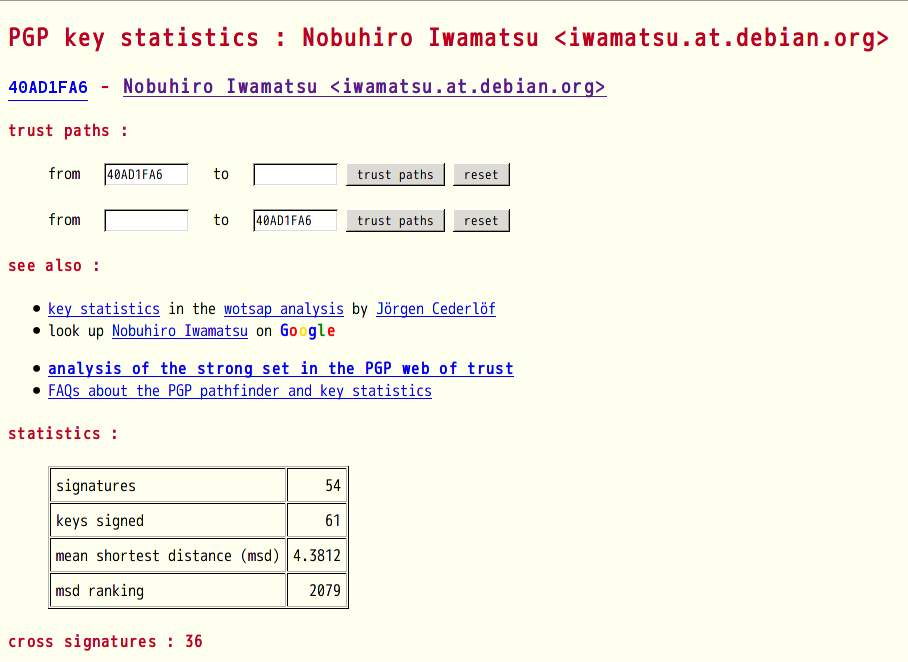
\includegraphics[width=0.8\hsize]{image200909/trust-path.png}
\end{center}
\end{frame}

\begin{frame}[containsverbatim]{Joerg$B$H4d>>$N(B trust path}
\begin{center}
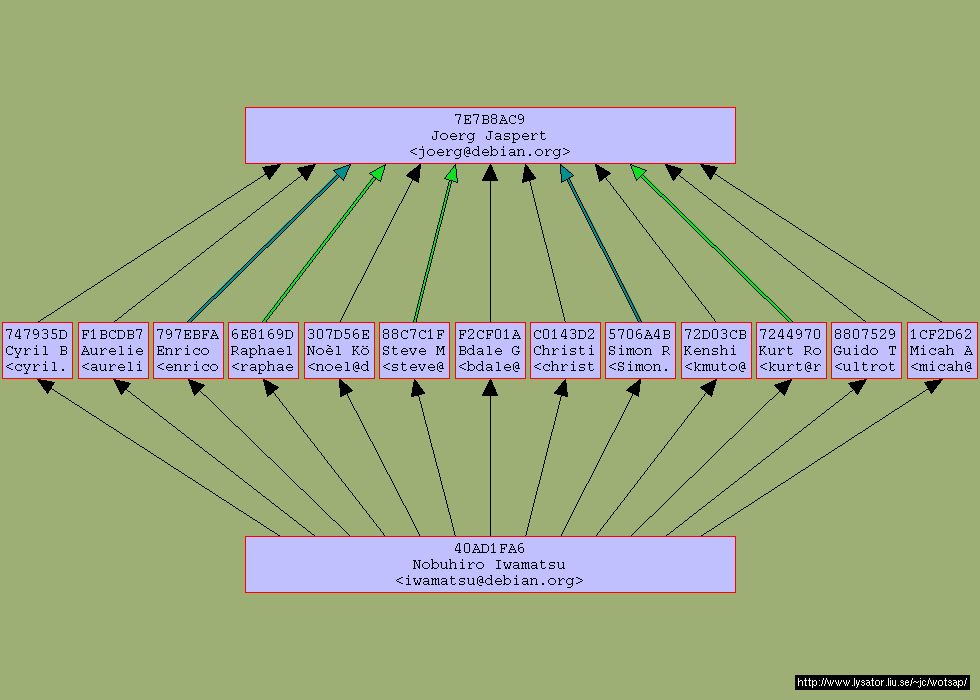
\includegraphics[width=0.8\hsize]{image200909/0x40AD1FA6-0x7E7B8AC9.png}
\end{center}
$BB>$N?M$r2p$7$F!"(BWeb of Trust $B$,$D$J$,$C$F$$$k$3$H$,J,$+$k!#(B
$BCN$j9g$$$NCN$j9g$$$,%5%$%s$7$F$$$k$h$&$@!#$A$g$C$H$O?.MQ$G$-$k$+$J!)$H$+!#(B
\end{frame}

\begin{frame}{$B%-!<%5%$%s$NN.$l(B}
\begin{center}
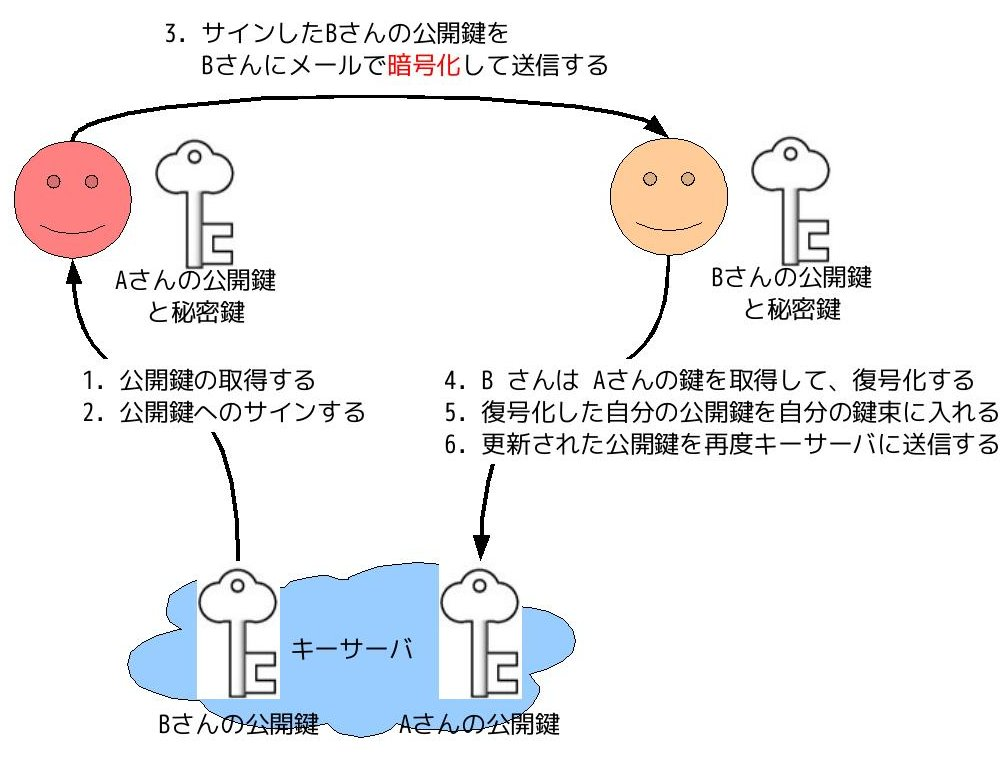
\includegraphics[width=1\hsize]{image200909/gpg-key.jpg}
\end{center}
\end{frame}

\begin{frame}[containsverbatim]{gpg $B%3%^%s%I$G$d$C$?>l9g(B}
\begin{commandline}
$ gpg --keyserver pgp.mit.edu --recv-key 40AD1FA6
$ gpg --fingerprint 40AD1FA6
$ gpg --edit-key 40AD1FA6
$ gpg --sign-key 40AD1FA6
$ gpg --check-sig 40AD1FA6                   
$ gpg --export -a 40AD1FA6 > iwamatsu.gpgkey   
$ iwamatsu.gpgkey $B$r(B $BAj<j$K%a!<%k$K(B $B=pL>(B+$B0E9f2=$7$FAw?.(B
\end{commandline}
\Huge $B?t?M$J$i$$$$$1$I!"(B100$B?M$H$+$d$C$F$i$l$s!*(B
\end{frame}

\begin{frame}[containsverbatim]{$B%$%s%9%H!<%k!&=i4|2=(B}

{\Huge $B$=$3$G(Bcaff$B$NEP>l!#(B}

caff $B$O(B signing-party $B%Q%C%1!<%8$GDs6!$5$l$F$$$k!#(B
\begin{commandline}
$ sudo apt-get install signing-party
\end{commandline}
caff $B$r;H$&$?$a$N=i4|2=$r9T$&!#(B
caff $B$r0l2s<B9T$9$k$H!"=i4|%U%!%$%k$r:n@.$7$F$/$l$k!#(B
\begin{commandline} 
$ caff
.......
#
#Regards,
#{$owner}
#EOM

Please edit /home/hoge/.caffrc and run caff again.
\end{commandline}
\end{frame}

\begin{frame}[containsverbatim]{caff$B$N@_Dj(B}
\~{}/.caffrc $B$K$"$k(B $B@_Dj%U%!%$%k$r=$@5$9$k!#(B
\begin{commandline}
$ cat ~/.caffrc

$CONFIG{'owner'} = 'Nobuhiro Iwamatsu';
$CONFIG{'email'} = 'iwamatsu@debian.org';

$CONFIG{'keyid'} = [ qw{4121C7433170EBE9 32247FBB40AD1FA6} ]

# Additionally encrypt messages for these keyids
$CONFIG{'also-encrypt-to'} = [ qw{4121C7433170EBE9 32247FBB40AD1FA6} ]

# Mail template to use for the encrypted part
$CONFIG{'mail-template'} = << 'EOM'\maketitle#Hi,

please find attached the user id{(scalar @uids >= 2 ? 's' : '')}
{foreach $uid (@uids) {
    $OUT .= ``\t''.$uid.''\n'';
};}of your key {$key} signed by me.
......

\end{commandline}
\end{frame}

\begin{frame}[containsverbatim]{caff$B$N@_Dj(B}          

caff $B$N%G%U%)%k%H$N@_Dj$G$O!"(Bcert-digest-algo $B$,(B SHA1 $B$K$J$C$F$$$k$N$G!"(B
 \footnote{http://bugs.debian.org/cgi-bin/bugreport.cgi?bug=527944} SHA512$B$K(B
 $B@_Dj$9$k!#(B
\begin{commandline}
$ mkdir -p ~/.caff/gnupghome
$ chmod 700 ~/.caff/gnupghome
$ cat >> ~/.caff/gnupghome/gpg.conf
cert-digest-algo SHA512
personal-digest-preferences SHA512
EOF
\end{commandline}


$B$^$?!"%a!<%k$r;H$&$N$G!"%m!<%+%k!J:n6H$9$k%^%7%s!K$N(BSMTP$B$b@_Dj$7$F$*$/I,MW$,$"$k!#(B
\end{frame}

\begin{frame}[containsverbatim]{caff$B$r;H$C$?=pL>(B}
$B=pL>$9$k(BID $B$r%-!<%5!<%P$+$i<hF@$7!";XDj$7$?<+J,$N(BID$B$G=pL>$7$F$/$l$k!#(B
$B$=$7$F!"=pL>$7$?80$r0E9f2=$7$FAw?.$7$F$/$l$k!#(B

\begin{commandline}
$ caff -u $B<+J,$N(BID $B=pL>$9$k(BID .......
\end{commandline}

\end{frame}

\begin{frame}[containsverbatim]{$B=pL>40N;8e(B}
$B=pL>8e$N%G!<%?$O(B \~{}/.gnupg/pubring.gpg $B$G$O$J$/!"(B{\bf \~{}/.caff/gnupghome/pubring.gpg} $B$K3JG<(B
 $B$5$l$k!#$3$N80B+$r(B \~{}/gnupg/pubring.gpg $B$K(B $B<h$j9~$`!#(B
\begin{commandline}
$ gpg --import ~/.caff/gnupghome/pubring.gpg
\end{commandline}

$B<h$j9~$s$@$i!"<+J,$N80$r%-!<%5!<%P$KAw?.!#(B
\begin{commandline}
$ gpg --keyserver pgp.nic.ad.jp --send-keys $B<+J,$N(BID
$ gpg --keyserver pgp.mit.edu --send-keys $B<+J,$N(BID
\end{commandline}
\end{frame}

\begin{frame}{$B:G8e$K(B}
$BAj<j$K80$rAw$k$^$G$,%-!<%5%$%s%Q!<%F%#$G$9!#(B
$B$A$c$s$HAj<j$K=pL>$7$?80$rAw$j$^$7$g$&!#(B
\end{frame}

\end{document}

;;; Local Variables: ***
;;; outline-regexp: "\\([ 	]*\\\\\\(documentstyle\\|documentclass\\|emtext\\|section\\|begin{frame}\\)\\*?[ 	]*[[{]\\|[]+\\)" ***
;;; End: ***
